\documentclass[logo,reportComp]{thesis}
\usepackage[python,pseudo,linenum]{mypackage}
\usepackage{relsize}

\setcounter{secnumdepth}{4}
\titleformat{\paragraph}{\bfseries}{\alph{paragraph})~~}{0em}{}
\titlespacing*{\paragraph}{0pt}{0pt}{0pt}[0pt]

\title{多核程序设计}
\subtitle{作业二:计算高维空间中的最近邻}
\school{数据科学与计算机学院}
\author{陈鸿峥}
\classname{17大数据与人工智能}
\stunum{17341015}
\headercontext{多核程序设计作业}

\let\emph\relax % there's no \RedeclareTextFontCommand
\DeclareTextFontCommand{\emph}{\kaiti\em}
\AtBeginEnvironment{quote}{\kaiti\small}

\def\globalmem{\textcolor{black}{\kaiti 全局内存}}
\def\sharedmem{\textcolor{red}{\kaiti 共享内存}}
\def\constmem{\textcolor{blue}{\kaiti 常量内存}}
\def\register{\textcolor{orange}{\kaiti 寄存器}}

\begin{document}

\maketitle
\tableofcontents

\newpage

\section{题目描述}
计算高维空间中的最近邻(nearest neighbor)
\begin{itemize}
	\item 输入:查询点集,参考点集,空间维度$k$
	\item 输出:对每个查询点,输出参考点集中最近邻的序号
\end{itemize}

回答以下问题:
\begin{enumerate}
	\item 介绍程序整体逻辑,包含的函数,每个函数完成的内容。(10分)
	\begin{itemize}
		\item 对于核函数,应该说明每个线程块及每个线程所分配的任务
	\end{itemize}
	\item 解释程序中涉及哪些类型的存储器(如全局内存、共享内存等),并通过分析数据的访存模式及该存储器的特性说明为何使用该种存储器。(15分)
	\item 针对查询点集为$1$个点及$1024$个点给出两个版本,并说明设计逻辑(例如任务分配方式)的异同。
	如两个版本使用同一逻辑,需说明原因。(35分)
	\item 请给出一个基础版本(baseline)及至少一个优化版本。
	并分析说明每种优化对性能的影响。(40分)
	\begin{itemize}
		\item 具体得分根据优化难度(技巧及工作量)而定
	\end{itemize}
	\item 选做:使用空间划分数据结构加速查询(如KD-Tree,BVH-Tree)。(20分)
\end{enumerate}

\section{问题简答}
\begin{enumerate}
	\item 参见第\ref{sec:imp}节,每个线程所做的任务均用加粗字体标注。
	\item 参见第\ref{sec:imp}节GPU共享内存、Warp原语版本等,不同类型的存储器均使用不同颜色字体进行标注。
	\item 参见第\ref{sec:imp}节,除了GPU Block归约版本,其他GPU优化版本对于查询点集为$1$个点和$1024$个点的任务分配方式均相同,但具体每个线程做的任务有所不同,可见下文加粗字体。
	基本的分配策略都是开设$m$个Block给$m$个查询点使用,而每个Block内的每个线程则用于计算每个参考点到该查询点的距离。
	这样的好处在于查询点的坐标可以直接存储在\sharedmem中,供所有参考点使用;并且所有的并行归约操作都限制在一个Block内,可以直接通过\sharedmem传输数据,而无需通过\globalmem,大大降低了访存的开销。
	\item 参见第\ref{sec:imp}节,一共实现了五个版本的GPU程序进行优化与比较,实验结果见第\ref{sec:exp}节。
\end{enumerate}

\section{具体实现}
\label{sec:imp}
本次实验我总共实现了六个版本的程序,包括CPU版本、GPU基线版本、GPU共享内存版本、GPU并行归约版本、GPU Warp原语版本,GPU Block归约版本。

\subsection{CPU版本}
最基础的实现即助教提供的CPU版本程序,依次遍历所有的查询点,对于每一个查询点,遍历所有的参考点,并(遍历每个维度)计算每个查询点和参考点之间的距离。
从这些距离中选取最小的,其下标即为所求的最近邻。

\lstinputlisting[language=c++,firstline=14,lastline=53]{../sources/src/core.cu}

\subsection{GPU基线版本}
GPU基线(baseline)版本即将CPU版本的最外层循环进行并行。
\textbf{每个线程处理一个查询点},同样是遍历所有的参考点并计算查询点与参考点之间的距离。
每个线程都各自计算出所有参考点的最小距离,并将结果直接写入\globalmem中。
核函数如下所示。
\lstinputlisting[language=c++,firstline=55,lastline=87]{../sources/src/core.cu}

GPU调用的接口如下所示,主要分为几个步骤:
\begin{enumerate}
	\item 为查询点坐标、参考点坐标、输出位置分配GPU内存
	\item 将查询点坐标、参考点坐标从主机端(CPU)传到设备端(GPU)
	\item 调用核函数,可以看到开设了$1$个Block,并且有$m$个线程。
	\item 将结果从GPU运回CPU
	\item 释放GPU内存
\end{enumerate}
\lstinputlisting[language=c++,firstline=89,lastline=129]{../sources/src/core.cu}

注释中的部分最开始用于核验CPU版本的程序与GPU版本程序的正确性。

\subsection{GPU共享内存版本}
注意到由于每次计算距离时都会涉及到\textbf{查询点集的大量内存访问},因此一个优化思路即将查询点集放置在\sharedmem中;至于参考点集则仍放置在\globalmem中,因为每个点坐标只会被访问一次,将其读取至\sharedmem也不会减少访问时间。

因此这里\textbf{每个Block计算一个查询点的最近邻,每个Thread分别计算$q$个参考点与查询点的距离}。
由于使用的GPU每个Block的最大线程数为$1024$,故$q=\lceil m/1024\rceil$。
具体流程如下:
\begin{itemize}
	\item 每个Block先开取$k$个线程,读取查询点的$k$维坐标向量到\sharedmem\verb's_mem'中
	\item 创建\sharedmem\verb'dist'和\verb'dist_idx'分别存储该Block内的最小距离值及其下标。
	注意到每个线程处理$q$个参考点,因此\verb'dist'和\verb'dist_idx'中的元素对应的也是这$q$个点的最小距离值及其下标(由于同个Block中的所有线程处理的是同个查询点,因此距离数组无需在Block之间传递,而可以采用\sharedmem方式实现)。
	\item 使用单一线程进行归约操作,对\verb'dist'数组进行遍历,寻找其中的最小值
	\item 每个Block将最终结果(距离最小值对应坐标)写入全局数组\verb'output'中
\end{itemize}

完整核函数代码如下所示。
\lstinputlisting[language=c++,firstline=142,lastline=185]{../sources/src/core.cu}

\subsection{GPU并行归约版本}
在上述\sharedmem版本的基础上,添加并行归约的功能。
需要在$1024$个元素中找最小值,这个可以采用树形的方式进行归约,如图\ref{fig:reduction}所示。
\begin{figure}[H]
\centering
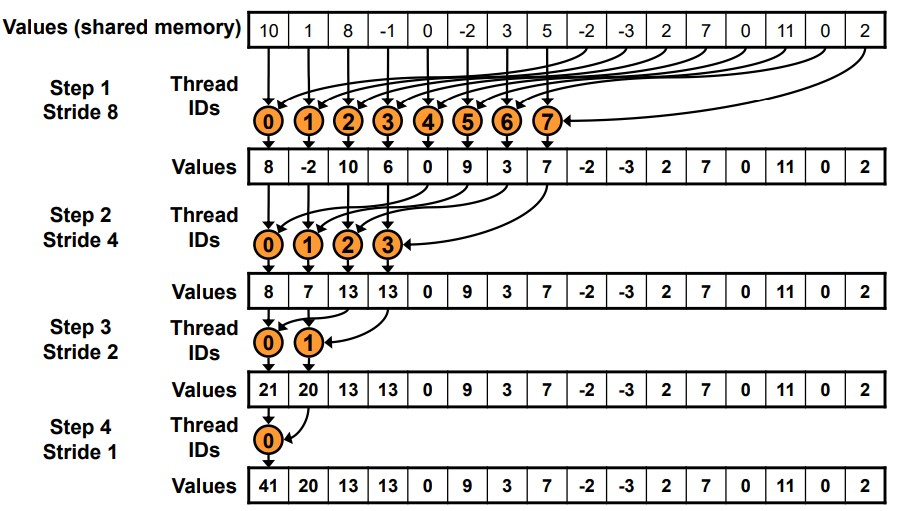
\includegraphics[width=0.8\linewidth]{fig/reduction.jpg}
\caption{树形方式归约}
\label{fig:reduction}
\end{figure}

注意这里读取的都是连续内存,通过加步长来消除存储体冲突。
每个线程计算两个元素间的最小值,最终$1024$个元素的最小值会被存放在数组第一个元素中。
由于全程的操作都在\sharedmem中完成,因此速度非常快。
最后只有一次\globalmem的写操作,即将最终结果写入\verb'output'中。

核函数并行归约部分代码如下所示。
\lstinputlisting[language=c++,firstline=271,lastline=283]{../sources/src/core.cu}
为确保参考点数目小于$1024$时也能够正常执行,这里的判断条件还添加了对$n$与步长关系的判断。
不过这个程序一个小缺陷在于只能支持$2$的指数次幂的归约。

\subsection{GPU Warp原语版本}
这里同样是对归约部分进行优化,由于采用树形归约方式,当线程数少于$32$时,就只剩第一个线程束(warp)还在工作了。
因此这时候可以直接采用线程束内的并行机制,在课件中可以通过展开最后一个线程束而无需添加\verb'__syncthreads'来实现并行归约求和。
但是对于求最小值这种涉及到判断语句的归约,则没有办法简单通过上述方法实现自动同步,否则会导致结果运算错误。

故解决方案是采用warp层面的原语操作,如图\ref{fig:shfl_down}所示,CUDA 9引入了几个新的原语,使得并行归约操作变得更加高效便捷。
对于一个线程束内的32个线程,\verb'__shfl_down_sync'可以实现线程之间的数据传输直接通过\register进行。
通过指定掩码、传输变量及偏移量,即可在线程束内实现快速高效的数据交换,进而达成归约的目的。
\begin{figure}[H]
\centering
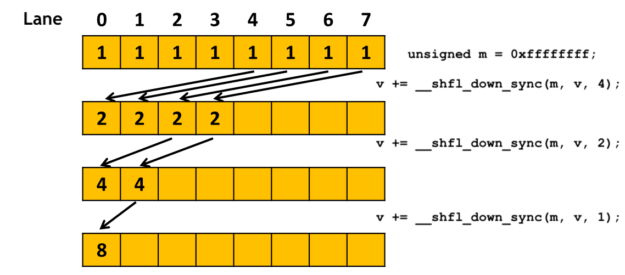
\includegraphics[width=0.8\linewidth]{fig/reduce_shfl_down.png}
\caption{\_\_shfl\_down\_sync原语操作}
\label{fig:shfl_down}
\end{figure}

具体到本问题来说,我将最后一个线程束进行包裹,实现了\verb'warpReduceMin'函数,同样是树形归约,但直接将高位线程数据搬移至低位线程求最小值,而不用再计算对应数组地址。
\lstinputlisting[language=c++,firstline=328,lastline=338]{../sources/src/core.cu}

注意到这里无需显式同步,而且数据直接通过\register交换,速度也会大幅提升。

核函数部分修改为下面代码。
\lstinputlisting[language=c++,firstline=382,lastline=396]{../sources/src/core.cu}

\subsection{GPU Block归约版本}
有了warp内的归约求最值,更进一步,可以将一个block内的所有warp都按照这种方式实现,这样将大幅减少\sharedmem的访问,同时也减少线程之间的同步。

故有下列\verb'blockReduceMin'函数,如果一个block内有$1024$个线程,那么将有$32$个wrap。
对每个wrap先调用\verb'warpReduceMin'求出每个wrap的最小值,然后再对这$32$个最小值求全局最小。
最后0号线程的结果即为全局最小值。
\lstinputlisting[language=c++,firstline=441,lastline=470]{../sources/src/core.cu}

注意如果参考点集小于1024个,则会回滚回Warp原语的版本,即只对最后一个线程束进行归约求最小值。

\section{实验设置与结果}
\label{sec:exp}
\subsection{环境设置}
为了避免占用学院集群环境的大量资源,我采用了另外一台服务器进行测试。
该服务器上装备了2个Intel Xeon Gold 5118处理器(24物理核/48逻辑核),另有一块Titan V GPU。
操作系统为Ubuntu 18.04 LTS,编译器采用gcc 7.4.0和nvcc 10.2。
同时,我也在学院集群上进行了简单测试,运行时间均与下述在服务器上的测试差异不大。

所有版本的正确性均已测试通过,下列所有实验均为运行多次取平均的结果。

\subsection{实验结果}
\label{sub:exp}
实验结果如图\ref{fig:cuda}所示,可以看到CPU版本的程序在样例较小时表现都比较好,但是一旦查询/参考点的数目提升了,其性能就下降得很快,与GPU优化后的版本差了2个数量级。

另外,可以看到\sharedmem的使用给GPU的性能带来了极大的提升,至少是1个数量级的优化。
GPU Baseline第一组数据的突起是由于冷启动造成的,后面GPU程序的运行则没有这种问题。

由于本次实验提供的测试样例规模依然较小,因此采用了不同归约优化方式,性能提升在图中看并不明显。
但是从完整实验数据(见附录\ref{appendix:exp})中可以看出无论是并行归约,还是采用warp原语,对GPU性能的影响依然是非常正面的。

\begin{figure}[H]
\centering
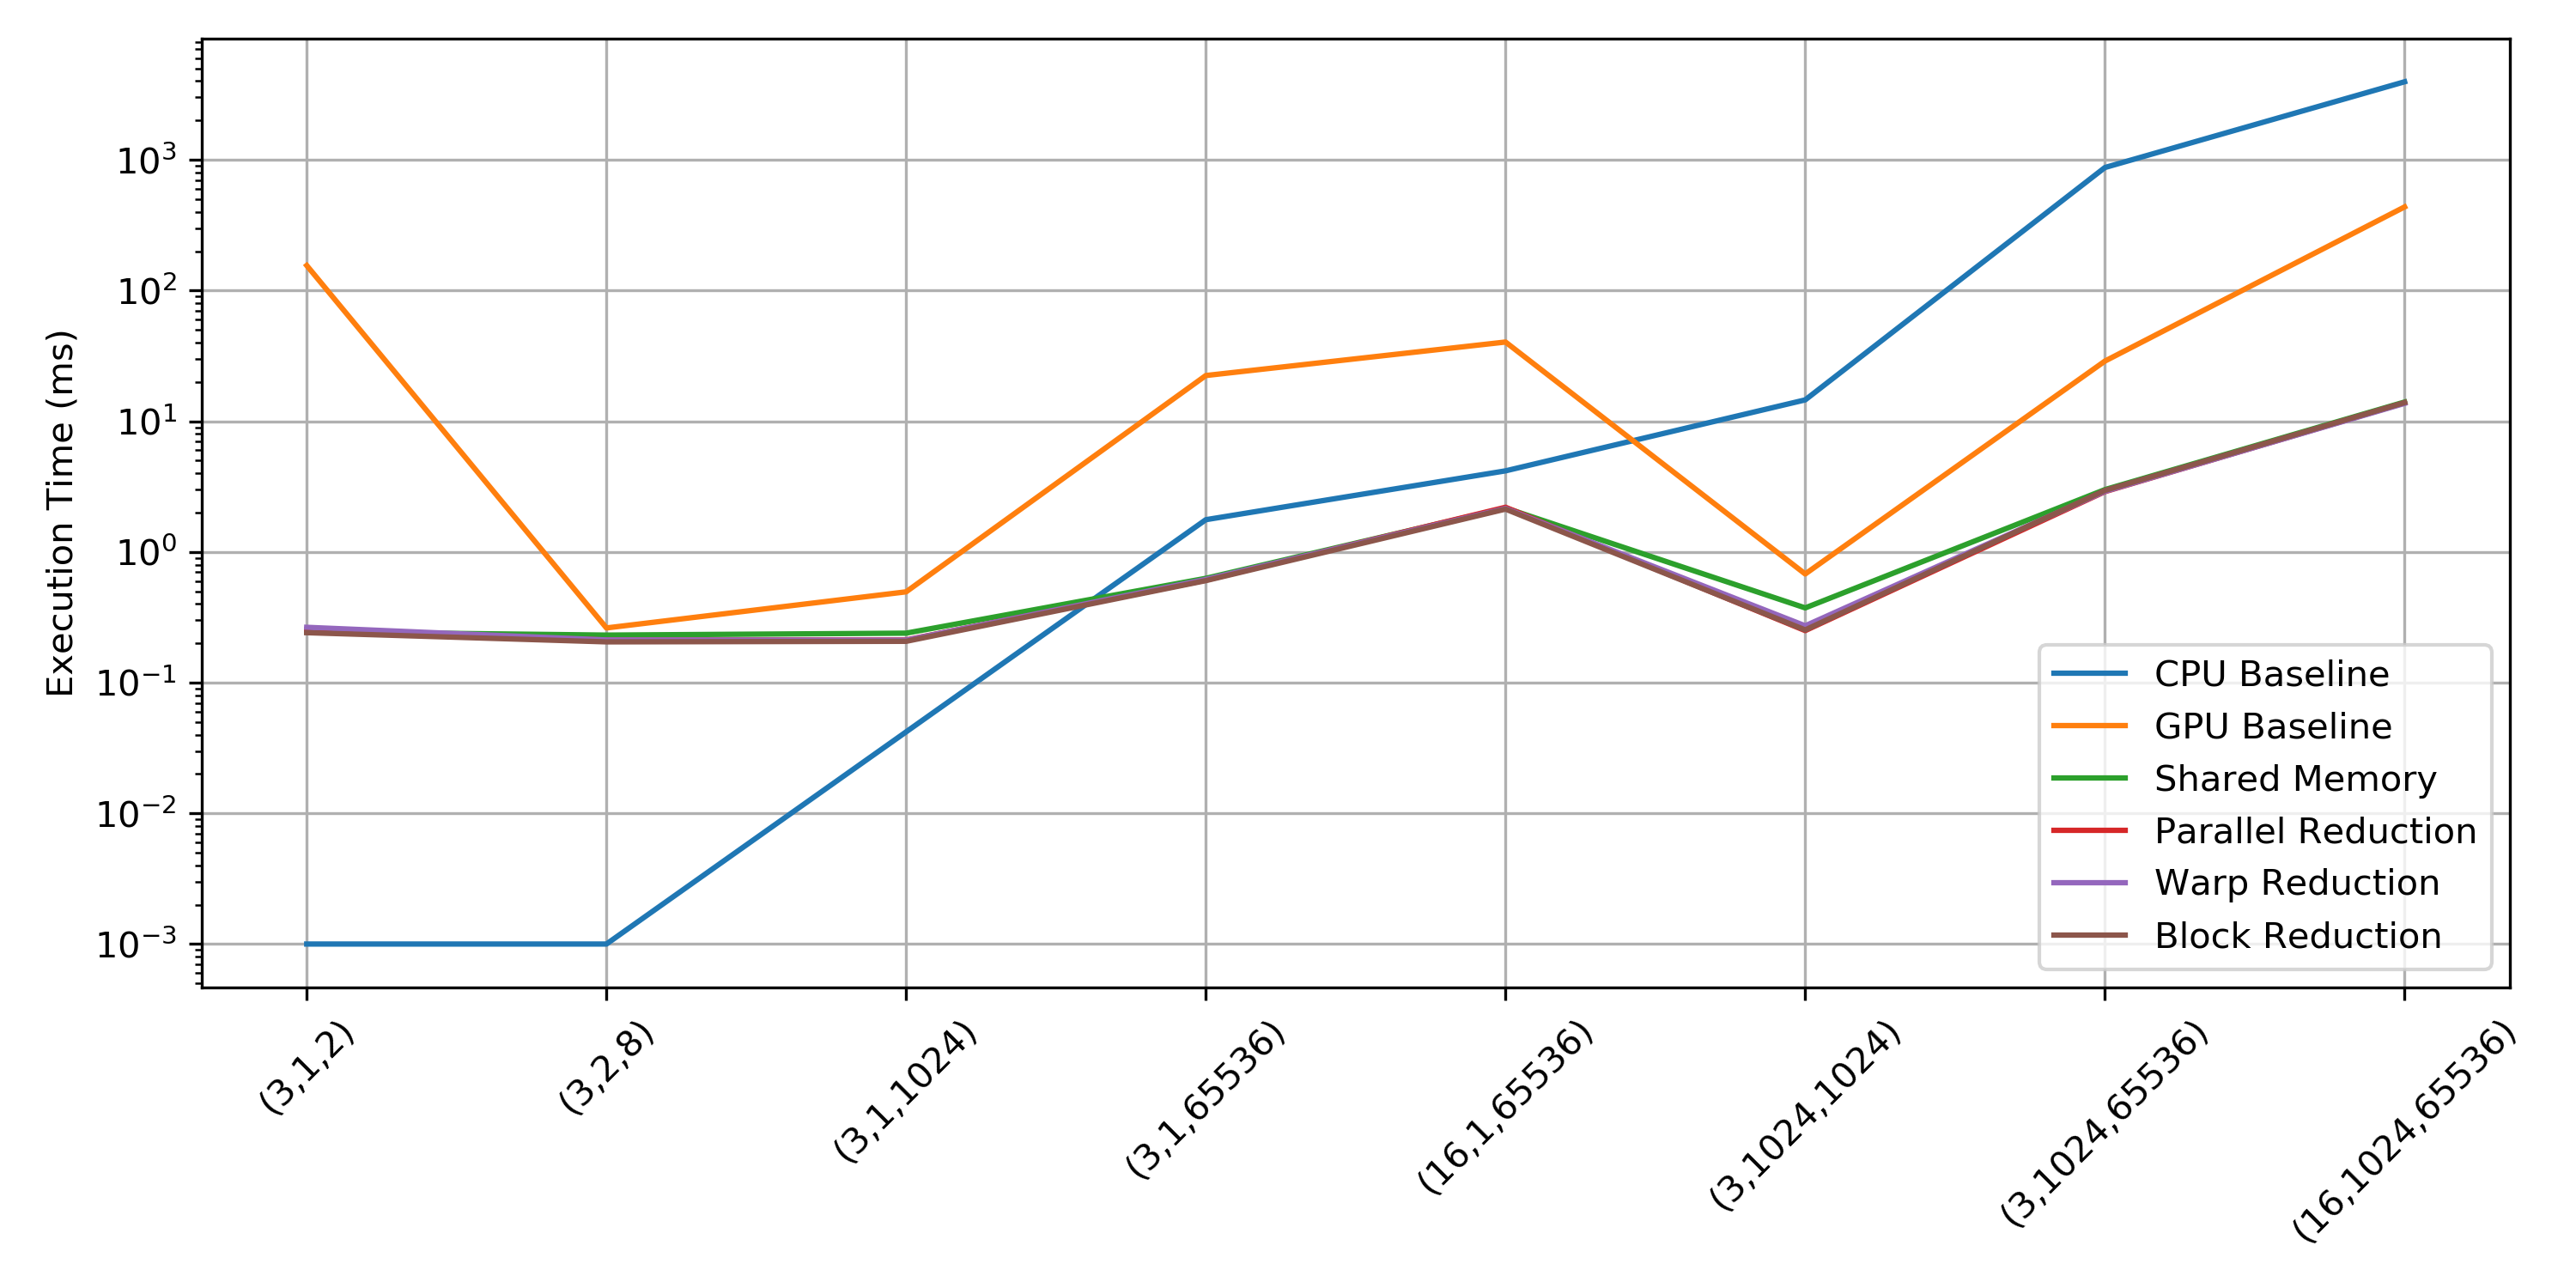
\includegraphics[width=\linewidth]{fig/cuda.png}
\caption{CUDA不同优化版本比较}
\label{fig:cuda}
\end{figure}

% \begin{thebibliography}{99}
% https://github.com/lkawka/3d-nearest-neighbor-search-in-kd-tree-cuda/blob/master/nn.cu
% http://cuda-programming.blogspot.com/2013/02/texture-memory-in-cuda-what-is-texture.html
% https://www.nvidia.com/content/gtc-2010/pdfs/2140_gtc2010.pdf
% http://vincentfpgarcia.github.io/kNN-CUDA/
% https://github.com/vincentfpgarcia/kNN-CUDA
% https://developer.nvidia.com/blog/using-cuda-warp-level-primitives/
% https://stackoverflow.com/questions/41996828/cuda-reduction-minimum-value-and-index
% \end{thebibliography}

\appendix
\appendixconfig
\section{完整实验数据}
\label{appendix:exp}
\begin{table}[H]
\centering
\caption{不同规模数据下不同版本程序的运行时间(ms)}
\scriptsize
\begin{tabular}{ccccccccc}\hline
 & (3,1,2) & (3,2,8) & (3,1,1024) & (3,1,65536) & (16,1,65536) & (3,1024,1024) & (3,1024,65536) & (16,1024,65536)\\\hline
CPU基线 & 0.001 & 0.001 & 0.042 & 1.764 & 4.171 & 14.559 & 872.909 & 3955.051\\\hline
GPU基线 & 155.364 & 0.262 & 0.495 & 22.362 & 40.349 & 0.678 & 28.838 & 436.137\\\hline
GPU共享内存 & 0.245 & 0.231 & 0.239 & 0.628 & 2.168 & 0.373 & 2.997 & 14.024\\\hline
GPU并行归约 & 0.253 & 0.212 & 0.212 & 0.608 & 2.196 & 0.250 & 2.891 & 13.815\\\hline
GPU Warp原语 & 0.265 & 0.212 & 0.211 & 0.616 & 2.149 & 0.272 & 2.909 & 13.696\\\hline
GPU Block归约 & 0.241 & 0.205 & 0.207 & 0.603 & 2.126 & 0.253 & 2.956 & 13.892\\\hline
\end{tabular}
\end{table}

\end{document}

% 评分细则
% – 程序正确性 40
% – 编程规范 10
% • 初始分 10
% • 缺少文件头 -5
% • 缺少函数头 -5
% • 换行没有正确缩进 -5
% • 函数过长 -5
% – 书面报告 100

% 提交作业
% – 邮箱:
% multicoresysu2020@163.com
% – 截止时间
% • 7月26日晚23:59
% • 如需使用slip days,请于截止时间前将需要使用的天数发送至提交作业邮箱

% 提交文件结构说明
% – your name-your ID
% • README (实验报告)
% • sources
% – all sources files
% – Makefile

% CUDA_VISIBLE_DEVICES=1 ./cuda_executable